\documentclass{article} % [twocolumn]
\usepackage[top=1.1in, left=0.85in, right=0.85in]{geometry}

% \usepackage{eclbkbox}
\usepackage{amsmath}
\usepackage{amssymb}
% \usepackage{amscd}
% \usepackage{xy}
\usepackage{graphicx}
% \usepackage{fancyhdr}
% \usepackage{color}
% \usepackage[dark,all,bottom,landscape,timestamp]{draftcopy}
% \usepackage{everypage}

% \usepackage{ulem}
% go back to italics for emphasis, though
% \normalem

\begin{document} 

\title{Who is the biggest douche in Skymall?}
\author{Dr.~Tom~Murphy~VII~Ph.D.\thanks{
Copyright \copyright\ 2011 the Regents of the Wikiplia
Foundation. Appears in SIGBOVIK 2011 with the blessing of the
Association for Computational Heresy; {\em IEEEEEE!} press,
Verlag-Verlag volume no.~0x40-2A.
\yen 0.00}
}

\date{1 April 2011}

\maketitle

\begin{abstract}
Did you ever notice how there are so many douches in the Skymall
catalog? This paper investigates the 22 males pictured in the January
2011 issue, using Internet technology to determine their douchiness.
We then present an efficient image recognition algorithm that reliably
predicts douchiness from photos.
\end{abstract}

\vspace{1em}
{\noindent \small {\bf Keywords}:
 computational douchebaggery, as seen on tv, man who can sleep in any seat
}

\section*{Introduction}
In that Luddite void between closing the cabin doors and the beep
indicating it is now safe to use approved electronic devices, there is
one perfect pleasure: The Skymall catalog. It has everything,
including: Pointlessly impractical products you cringe at just
imagining someone receiving as unwanted gifts at Christmas, copy that
preys on the insecurities of business travelers, typo and physically
impossible hyperbole treasure hunts galore, Photoshop disasters, new
friends, and old familiar faces. But since 1990, science has wondered:
{\bf Who is the biggest douche in Skymall?}

It is difficult to assess the absolute douchiness (say, on a scale
from 1 to 10) of a given person. So, in order to answer this question,
we used Internet Technology to conduct a series of
more-douche--less-douche battles between randomly selected pairs of
participants. The visitor is simply asked: Who is the bigger douche?
The proportion of battles won, overall, is the final douche score.

After thousands of battles waged, we converged on the following results,
ranked in descending douchiness:

\section*{Results}

\newcommand\douche[6]{
  \begin{minipage}{0.332 \linewidth}
  \includegraphics[width=#1 \linewidth]{#2} \\
  \raggedright
  {\bf #3} \\
  {\small won #4/#5;} #6\% douche
  \end{minipage}
}

\douche{0.45}{personal-headphones}{In Charge of the Music}{207}{66}{75.82}
\douche{0.45}{head-spa-massage}{The Thinker}{201}{73}{73.35}
\douche{0.75}{sandproof-blanket}{Seaside Date}{197}{76}{72.16}
\douche{0.75}{laptop-holder}{Reclining Numbercruncher}{193}{80}{70.69}
\douche{0.75}{fluidity-of-motion}{Karate Genius}{188}{85}{68.86}
\douche{0.75}{poolside-read}{Poolside Bibliophile}{177}{95}{65.07}
\douche{0.75}{global-network}{Traveling Salesman}{171}{102}{62.63}
\douche{0.75}{relaxing}{Beauty Rest}{167}{106}{61.17}
\douche{0.75}{jeweler}{Jeweler}{167}{106}{61.17}
\douche{0.75}{i-have-to-take-this}{I Have to Take This}{161}{113}{58.75}
\douche{0.75}{nose-jewelry}{Cured Snorer}{141}{132}{51.64}
\douche{0.75}{sleeping}{Man who can Sleep in Any Seat}{131}{141}{48.16}
\douche{0.75}{after}{Treatment Recipent}{121}{152}{44.32}
\douche{0.55}{business-expert}{Business Expert}{118}{155}{43.22}
\douche{0.75}{confidence}{Confident in Glasses}{118}{155}{43.22}
\douche{0.75}{sass-moulavi}{Sass Moulavi, M.D.}{117}{155}{43.01}
\douche{0.55}{videochat}{New Haircut}{96}{177}{35.16}
\douche{0.45}{pockets-jacket}{Woodsy Gentleman}{86}{186}{31.61}
\douche{0.75}{john-q-storus}{John Q. Storus}{78}{195}{28.57}
\douche{0.45}{security-system}{Father/Kidnapper}{73}{199}{26.83}
\douche{0.55}{promotion}{Got the Promotion}{59}{214}{21.61}
\douche{0.45}{runner}{Silver Medalist}{34}{238}{12.50}

Although many people disagreed on the finer points of what constitutes
a douche, the results were fairly significant, in that there were many
participants that were consistently perceived as more or less douchey.
This is truly a victory for the scientific method. Speaking of
victories:

\section*{Douche recognition}

Having collected consensus on what constitutes a douche, we next turn
to the problem of determining whether any given person is a douche,
even if that person has not participated in hundreds of rounds of
douche-battle. Since people appear to be able to make decisions based
mainly on images, we look to image processing techniques.

Images are formed using ``pixels'', which are like tiny individual
color dots. Each color dot, or ``pixel'', is saved in a file. It turns
out that these files are all the same one: Every ``pixel'' is in a
file, which constitutes the series of color dots, as a series of bytes
or ``1s and 0s''~\ref{fig:ones}, which constitute the digital
information that is the file, or ``pixels.'' Point is, in order for a
computer to ``see'' a file, all it needs to do is look at it, by
rubbing the files and ``pixels'' on its CPUs, the same way that you or
I look at a picture by rubbing it on our eyeballs.

The problem with most image recognition algorithms is that they do not
work, and are also slow.

We eschew the traditional model-based approaches, instead using efficient
hashing algorithms such as SHA-1 and MD5. These operate directly on
the ``1s and 0s'' of the image, and run in linear time. This way, even
if the algorithms do not work, they will at least be fast.

We find that the algorithm SHA-1 correlates with the douchiness of the
image, but not well. The MD5 algorithm is faster but in fact correlates
negatively. However, by fine tuning the initialization vector, we are
able to produce a variant that is just as fast and correlates very well
with the data (Figure~\ref{fig:chart}).

\begin{figure*}
\begin{center}
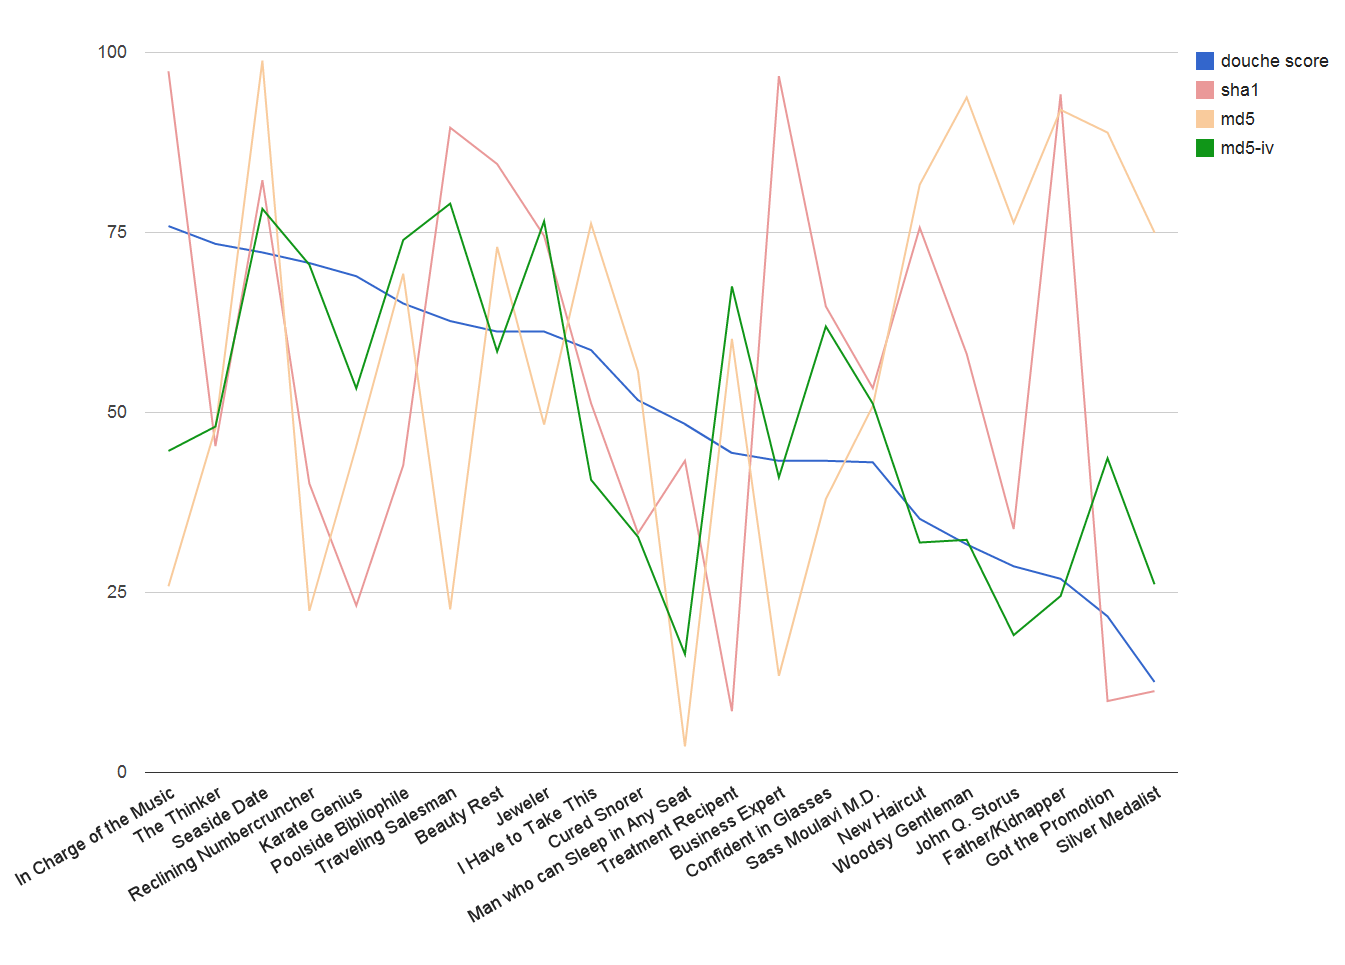
\includegraphics[width=0.9 \linewidth]{chart}
\end{center}\vspace{-0.1in}
\caption{Performance of different prediction algorithms. SHA-1
  correlates with the douchiness of the image, though it tends to
  overestimate the douchiness of medium-low douches. MD5 actually
  has negative correlation. A tuned variant of MD5 with the
  initialization vector {\tt A8F82303 08A1B76B AA25DA9E 4C2C1883}
  correlates quite neatly.}
\label{fig:chart}
\end{figure*}

\section*{Conclusion}
Do you disagree with these data (Y/n)? If (Y), then Science never Sleeps!
{\tt http://snoot.org/toys/wuss/skymall/}

\begin{figure}
\begin{center}
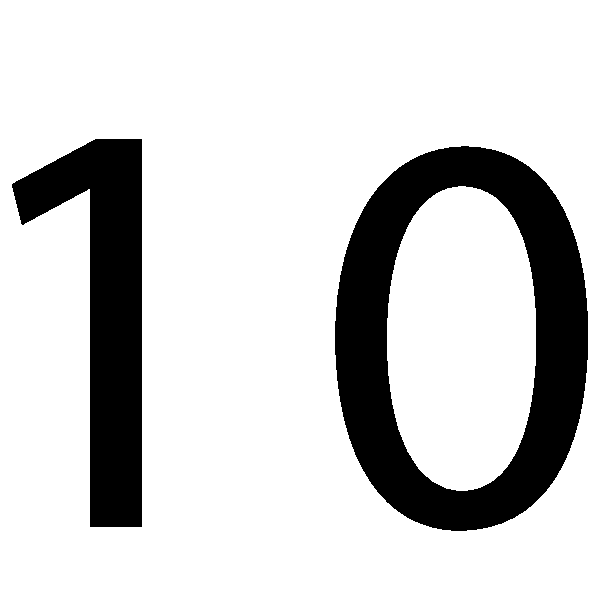
\includegraphics[width=0.15 \linewidth]{ones}
\end{center}\vspace{-0.1in}
\caption{Image files consist of ``ones'' or ``zeroes'', which is
  digital information pixels (pictured).}
\label{fig:ones}
\end{figure}

\section*{Poolside Bibliography}
Sorry, I didn't read any papers or anything or do actual science.

\end{document}
